\newpage
\section{Conceitos e Tecnologias Utilizadas}

\par Este capítulo aborda os conceitos e as tecnologias que sustentam o trabalho: automação industrial, tecnologia da informação aplicada ao contexto industrial e desenvolvimento de software. O objetivo é reunir definições, enquadramentos e ferramentas necessários para compreender, nas seções seguintes, a proposta de sistema supervisório web orientado a serviços, explicitando como cada tema se articula com a solução adotada.

\subsection{Sistema SCADA}

\par A indústria evoluiu muito na busca por mais monitoramento e controle dos processos. Com o tempo, os custos de computadores, hubs e conversores de rede caíram bastante, ao passo que o desenvolvimento de software ganhava relevância. Nesse contexto, as empresas de software industrial passaram a oferecer soluções personalizadas para cada tipo de processo e indústria, com ampla gama de protocolos de comunicação. A esse tipo de sistema deu-se o nome de SCADA, sigla em inglês para \emph{Supervisory Control and Data Acquisition} \cite{ZANGHI2019_SCADA_CONCEITOS}. De forma geral, define-se o SCADA como um pacote de software posicionado sobre o hardware ao qual se interliga, que viabiliza a supervisão e o controle de processos industriais de forma local ou remota \cite{PHUYAL2020_COST_EFFICIENT_SCADA, AHMED2011_EFFICIENT_WEB_SCADA}.

\par Para \textcite{ZANGHI2019_SCADA_CONCEITOS}, um sistema SCADA deve contemplar seis módulos, descritos nas subseções a seguir: aquisição e registro de dados, sincronismo de tempo, níveis de acesso, comando e controle, escalabilidade e redundância.

\subsubsection{Aquisição e Registro de Dados}

\par A aquisição das informações de campo é o primeiro grande desafio em um sistema SCADA \cite{ZANGHI2019_SCADA_CONCEITOS}. Atualmente, predominam dispositivos genéricos inteligentes que disponibilizam algum protocolo de comunicação, responsáveis por adquirir grandezas analógicas e digitais e disponibilizá-las ao supervisório em formato binário por meio de uma rede de dados \cite{YADAV2020_SCADA_ARCHITECTURE_REVIEW}. O meio de comunicação varia conforme a distância e a infraestrutura disponível, indo das redes locais cabeadas, tipicamente Ethernet, a enlaces sem fio como rádio frequência (RF) e telefonia móvel (4G) \cite{STOUFFER2015_NIST_ICS_SECURITY}, até soluções orientadas à Internet das Coisas, que trafegam os dados pela internet \cite{KHALID2024_IOT_SCADA_PHOTOVOLTAIC}.

\par Os pontos aquisitados em um sistema SCADA são denominados \emph{tags} e armazenados no banco de dados do supervisório. Cada \emph{tag} assume um tipo de dado conforme a natureza da grandeza que representa, podendo ser booleano, inteiro, real ou texto. O registro contínuo desses valores pelo supervisório permite análises posteriores, na forma de gráficos históricos de tendência e de sequenciais de eventos \cite{ZANGHI2019_SCADA_CONCEITOS}.

\subsubsection{Sincronismo de Tempo}

\par Outro requisito fundamental dos sistemas SCADA é o sincronismo de tempo. Todo dado coletado deve possuir um registro de tempo de origem, a chamada estampa de tempo (\emph{time stamp}), de modo que cada variação de estado fique associada a um instante de referência. Essa exigência decorre da necessidade de análises posteriores de ocorrências e faltas, que dependem da cronologia precisa dos acontecimentos para permitir a identificação das causas \cite{ZANGHI2019_SCADA_CONCEITOS}.

\par Na prática, a aquisição é realizada de forma cíclica: o supervisório consulta periodicamente os dispositivos de campo, processo conhecido como \emph{polling} \cite{STOUFFER2015_NIST_ICS_SECURITY}, em ciclos de leitura sucessivos cuja frequência é definida conforme a dinâmica do processo \cite{YADAV2020_SCADA_ARCHITECTURE_REVIEW}. Como consequência, a estampa de tempo atribuída a cada ponto corresponde ao ciclo em que o valor foi lido, e não ao instante físico exato da transição, de modo que a resolução temporal do registro fica limitada ao período do ciclo de aquisição.

\subsubsection{Níveis de Acesso}

\par Os níveis de acesso de um sistema SCADA definem a separação das permissões de supervisão e controle entre os usuários. Classicamente organizada em níveis por instalação \cite{ZANGHI2019_SCADA_CONCEITOS}, essa separação materializa-se como acessos definidos por planta, em que cada usuário recebe permissões apenas sobre os pontos e comandos da instalação à qual está vinculado, segundo o controle de acesso baseado em cargos e o princípio do menor privilégio, apoiado em mecanismos adequados de autenticação e autorização \cite{STOUFFER2015_NIST_ICS_SECURITY}.

\subsubsection{Comando e Controle}

\par As ações executadas remotamente pelo supervisório consistem no envio de comandos aos dispositivos de campo, isto é, na escrita de uma informação no dispositivo \cite{YADAV2020_SCADA_ARCHITECTURE_REVIEW}. Quanto ao momento de execução, o comando pode ser instantâneo, escrevendo de imediato o valor desejado ou agendado, programado para ações conforme cenários previamente definidos, com o instante de execução registrado \cite{ZANGHI2019_SCADA_CONCEITOS}.

\par O processamento de um comando segue quatro fases: seleção, em que o operador escolhe na interface o equipamento; verificação de intertravamentos e condições de segurança; confirmação explícita pelo operador; e execução, com o envio efetivo da ordem ao elemento final de controle \cite{ZANGHI2019_SCADA_CONCEITOS}. Após a execução, o supervisório verifica a confirmação para garantir que a solicitação foi aceita pelo dispositivo e, em caso de falha, gera um alarme, pois comandos indevidos podem danificar equipamentos ou comprometer a segurança do processo \cite{STOUFFER2015_NIST_ICS_SECURITY}.

\subsubsection{Escalabilidade}

\par A expansão das instalações é frequente em ambientes industriais, com a inclusão de novos equipamentos, pontos de medição e circuitos. Para acompanhá-la, o software SCADA deve ser escalável, permitindo acrescentar pontos à base de dados e criar novas telas de operação sem comprometer o que já está em produção \cite{ZANGHI2019_SCADA_CONCEITOS}.

\par A análise da escalabilidade deve abranger não apenas o supervisório, mas também os elementos de aquisição, controle e rede, que precisam permitir o acréscimo de novos dispositivos ao barramento de comunicação, integração a ser prevista já na fase inicial do projeto \cite{ZANGHI2019_SCADA_CONCEITOS}.

\subsubsection{Redundância}

\par A redundância consiste no acréscimo de um elemento idêntico ao original, de modo que, em caso de falha do primeiro, o segundo assuma suas funções da forma mais transparente possível para a operação \cite{ZANGHI2019_SCADA_CONCEITOS}. A prática aplica-se a diversos componentes do sistema, como softwares supervisórios, dispositivos de aquisição e controle e elementos de rede, apesar do custo adicional, eleva a confiabilidade a graus compatíveis com a criticidade de aplicações industriais sensíveis \cite{SALVADOR2019_AQUISICAO_REDUNDANCIA}.

\par Em uma arquitetura redundante típica, múltiplas estações de operação comunicam-se simultaneamente com os dispositivos de campo e as unidades de aquisição e controle operam em pares espelhados \cite{ZANGHI2019_SCADA_CONCEITOS}. De modo geral, recomenda-se que cada componente crítico tenha um par redundante, sobre redes igualmente redundantes, e que o sistema seja projetado para degradação suave, preservando a supervisão e o controle mesmo diante de falhas pontuais \cite{STOUFFER2015_NIST_ICS_SECURITY}.

\subsection{Automação e Tecnologias da Indústria 4.0}

\par A automação industrial é o conjunto de tecnologias e práticas que substituem a intervenção humana direta na execução de processos produtivos por sistemas eletrônicos, mecânicos e computacionais capazes de medir, controlar, comandar e supervisionar variáveis físicas. A informática industrial, por sua vez, designa a aplicação das tecnologias da informação e da comunicação a esse contexto, articulando o mundo da Tecnologia da Automação (TA), voltado a tempo real determinístico, robustez e segurança operacional, com o da Tecnologia da Informação (TI), orientado a interoperabilidade, escala e segurança da informação. \textcite{COLOMBO2014_STATE_ART_AUTOMATION} apontam a convergência entre TA e TI como um dos principais vetores de transformação da automação contemporânea, frequentemente descrita como o desfecho que conduz à Indústria 4.0 \cite{PISCHING2017,BIGHETI2020}.

\par A Internet das Coisas (\emph{Internet of Things}, IoT) é uma rede global que liga à internet objetos físicos e virtuais, cada um com identidade digital própria, capazes de trocar informações entre si sem intervenção humana \cite{PISCHING2017,BIGHETI2020}. Ela reúne em um mesmo ambiente tecnologias como a computação móvel, as redes de sensores sem fio e os sistemas ciber-físicos, apontando para um cenário em que medir e monitorar o mundo se torna tão corriqueiro quanto o uso da eletricidade \cite{STANKOVIC2014_IOT_RESEARCH_DIRECTIONS}. Por envolver de bilhões a trilhões de dispositivos, traz desafios de identificação, autenticação, confiabilidade, armazenamento e privacidade; e, como muitos desses dispositivos atuam diretamente sobre o mundo físico, uma falha passa a ser também uma questão de segurança operacional \cite{STANKOVIC2014_IOT_RESEARCH_DIRECTIONS}.

\par Quando esse paradigma é trazido para o domínio industrial, sensoriamento de processos, controle de máquinas e otimização de cadeias produtivas, recebe o nome de Internet Industrial das Coisas (\emph{Industrial Internet of Things}, IIoT), um subconjunto da IoT especializado para ampliar a eficiência e a responsividade das plantas \cite{BIGHETI2020}. Embora compartilhem o mesmo núcleo, a IoT de consumo e a IIoT diferem em criticidade: a primeira lida com cenários ad-hoc e requisitos brandos, enquanto a segunda envolve nós fixos, altos volumes de dados e exigências rigorosas de tempo real, confiabilidade e segurança \cite{BIGHETI2020}. Para \textcite{PISCHING2017}, a proliferação da IoT na indústria leva fabricantes a embarcar tecnologias que sustentam a convergência TA/TI; e, à medida que dispositivos de campo expõem suas funções como serviços de rede, por exemplo via OPC-UA, a pirâmide ISA-95 \cite{ISA95_2000_ENTERPRISE_CONTROL} tende a achatar-se em uma arquitetura logicamente plana baseada em serviços \cite{COLOMBO2014_STATE_ART_AUTOMATION}.

\par A base de comunicação que sustenta esses conceitos é a troca direta de informações entre dispositivos, denominada comunicação Máquina a Máquina (\emph{Machine-to-Machine}, M2M). Originada na telemetria industrial e nos primeiros sistemas SCADA, a M2M precede e fundamenta a IoT e viabiliza a noção de máquina inteligente: dispositivos que coordenam ações, ajustam parâmetros e reportam estados sem intervenção manual \cite{BIGHETI2020,PISCHING2017}. Tecnologicamente, apoia-se em uma família de protocolos, do Modbus, mais difundido em telemetria, ao MQTT, leve e do tipo publicador-assinante, e ao OPC-UA, que oferece um modelo unificado de informação para comunicação segura entre dispositivos heterogêneos \cite{COLOMBO2014_STATE_ART_AUTOMATION}. Em redes de longa distância, CLPs em campo comunicam-se por meio de modems celulares com \emph{gateways} que concentram sessões e roteiam requisições até os serviços em nuvem, permitindo supervisionar centenas de pontos remotos sem hardware proprietário em cada instalação.

\par Os Sistemas Ciber-Físicos (\emph{Cyber-Physical Systems}, CPS), termo proposto em 2006 nos Estados Unidos, descrevem o acoplamento intensivo entre entidades computacionais e o mundo físico \cite{PISCHING2017,MONOSTORI2016_CPS_MANUFACTURING}. Mais relevante que a soma das partes é a interseção entre os mundos físico e cibernético: é a interação entre eles que caracteriza o CPS \cite{MONOSTORI2016_CPS_MANUFACTURING}. Herdeiros dos sistemas embarcados, os CPS acrescentam conectividade, autonomia e cooperação, e no domínio da manufatura recebem o nome de sistemas ciber-físicos de produção. \textcite{MONOSTORI2016_CPS_MANUFACTURING} destacam três características essenciais: a inteligência, capacidade de adquirir informações do entorno e agir autonomamente; a conectividade, uso de conexões com outros elementos, pessoas e serviços; e a responsividade, reação em tempo apropriado a mudanças. Como observa \textcite{PISCHING2017}, os CPS oferecem a base física e computacional sobre a qual a IoT viabiliza a Indústria 4.0. A Figura~\ref{fig:venn_iot_iiot_cps_i40} sintetiza as relações entre esses conceitos: a IoT como universo mais amplo, a IIoT em sua interseção com o domínio industrial, os CPS como categoria de forte acoplamento computação-físico, e a Indústria 4.0 emergindo na interseção entre IIoT e CPS \cite{BIGHETI2020,PISCHING2017}.

\begin{figure}[H]
    \centering
    \caption{Interseções de IoT, CPS, IIoT e Indústria 4.0}
    \centering
    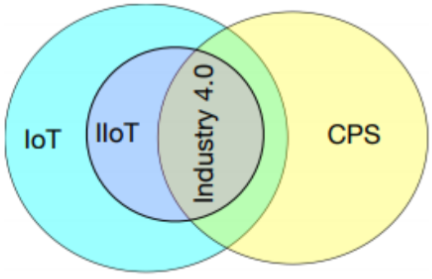
\includegraphics[width=0.9\textwidth]{Imagens/Desenvolvimento/Cap1/venn_iot_iiot_cps_i40-034.png}
    \centering
    \vspace{0.2cm} \\
    Fonte: \textcite[p.~27]{BIGHETI2020}.
    \label{fig:venn_iot_iiot_cps_i40}
\end{figure}

\par O termo \emph{Industrie 4.0} foi apresentado em 2011, na Feira de Hannover, e oficializado em 2013 pela estratégia de alta tecnologia do governo alemão, anunciando \emph{ex-ante} uma quarta revolução industrial \cite{PISCHING2017,BIGHETI2020}; reconhecimento que ganhou escala global quando o Fórum Econômico Mundial elegeu a quarta revolução industrial como tema central de sua reunião de 2016 \cite{WEF_DAVOS_2016_THEME}. \textcite{LASI_INDUSTRY_40} a caracterizam pela conjunção de um \emph{application-pull}, com demanda por personalização, flexibilidade e descentralização, e um \emph{technology-push}, fundado na automação crescente, na digitalização e na miniaturização do \textit{hardware}. \textcite{BIGHETI2020} a define como um conjunto de tecnologias coordenadas para conferir competitividade e customização, habilitadas por CPS, IIoT, computação em nuvem, redes sem fio e uso massivo de dados, cujo conceito-síntese é a fábrica inteligente. Seus princípios de projeto, segundo \textcite{PISCHING2017}, são a interoperabilidade, a virtualização, a descentralização, a operação em tempo real, a orientação a serviços e a modularidade, padronizados pelo modelo de referência RAMI 4.0. Nesse contexto, o SCADA deixa de ser um sistema fechado de supervisão local e passa a um nó de uma rede de serviços que integra produção, manutenção, logística e clientes em uma cadeia de valor digital \cite{BIGHETI2020,COLOMBO2014_STATE_ART_AUTOMATION}.

\subsection{Banco de Dados}

\par O banco de dados é o componente de software responsável por armazenar, organizar e recuperar informações de forma persistente. Quanto à organização dos dados, destacam-se dois grandes paradigmas: o relacional, que estrutura os dados em tabelas com esquema definido e relações explícitas entre as entidades, e o NoSQL, voltado a cenários de alta variabilidade de esquema e escala horizontal \cite{MOHAMED2014_RELATIONAL_VS_NOSQL}. Por organizar os dados de forma estruturada e preservar a integridade entre entidades relacionadas, o modelo relacional é o adequado a sistemas que exigem consistência e consultas expressivas, sendo o detalhado a seguir.

\par O modelo relacional, proposto por Edgar F. Codd em 1970 e materializado em bancos como PostgreSQL, MySQL e Oracle, organiza os dados em tabelas de linhas e colunas, cada uma definida por um esquema, uma chave primária que identifica unicamente cada registro e, opcionalmente, chaves estrangeiras que estabelecem relações entre tabelas, garantindo integridade referencial. A linguagem de consulta padrão é o SQL (\emph{Structured Query Language}), com operações de seleção, inserção, atualização e remoção, além de junções, agregações, transações e índices. Um exemplo amplamente adotado é o \emph{PostgreSQL}, banco relacional de código aberto com forte suporte a tipos complexos (JSON, \emph{arrays}), consultas em janelas de tempo e extensões para séries temporais \cite{POSTGRESQL_DOCS}.

\par Em ambientes de produção, boas práticas incluem indexar os campos mais consultados, particionar as tabelas históricas por intervalo de tempo para evitar tabelas monolíticas e empregar réplicas com \emph{failover} automático e \emph{snapshots} para alta disponibilidade \cite{DAMIN2022_MELHORES_PRATICAS_E3, SALVADOR2019_AQUISICAO_REDUNDANCIA}.

\subsection{Redis}

\par O \emph{Redis} é um armazenamento de dados em memória, de código aberto, que opera como banco chave-valor de altíssimo desempenho. Diferentemente dos bancos relacionais, em que a persistência em disco é a prioridade, o Redis mantém todo o conjunto de trabalho em memória RAM, oferecendo latências sub-milissegundo para operações de leitura e escrita  \cite{REDIS_DOCS}.

\par O Redis oferece persistência opcional por \emph{snapshots} periódicos e log de operações de escrita, expiração automática de chaves por \emph{time-to-live} (TTL) e um mecanismo publicador-assinante (Pub/Sub) para troca de mensagens entre processos. Por essas características, é comumente empregado como cache de acesso rápido, como barramento de eventos e como armazenamento de dados temporários \cite{REDIS_DOCS}.

\par Como o Redis guarda os dados em memória, ele usa cópias e recuperação automática para não parar diante de falhas. A replicação mantém uma ou mais réplicas sempre atualizadas da instância principal. Sobre isso, o \emph{Redis Sentinel} cuida da disponibilidade: vigia a instância principal e, se ela cai, promove sozinho uma réplica ao seu lugar, sem intervenção manual. Já o \emph{Redis Cluster} cuida do crescimento: reparte as chaves entre vários nós, de modo que basta acrescentar nós para aumentar a capacidade, e cada nó pode ter réplicas para o serviço continuar mesmo se um deles falhar \cite{REDIS_DOCS}.

\subsection{Docker}

\par O Docker é uma plataforma de virtualização baseada em contêineres, unidades de empacotamento que reúnem código, bibliotecas e dependências em um artefato portável \cite{DOCKER_DOCS}. Diferentemente das máquinas virtuais \cite{SALVADOR2019_VIRTUALIZACAO}, que emulam uma máquina inteira com seu sistema operacional, os contêineres compartilham o \emph{kernel} do hospedeiro e isolam apenas o espaço de processos e o sistema de arquivos da aplicação (Figura~\ref{fig:vm_vs_container}). Por isso são ordens de magnitude mais leves: enquanto uma máquina virtual pode levar minutos para iniciar e ocupar gigabytes, um contêiner inicia em segundos e consome dezenas a centenas de megabytes.

\begin{figure}[H]
    \centering
    \caption{Arquitetura comparada: máquinas virtuais (esquerda) e contêineres Docker (direita)}
    \label{fig:vm_vs_container}
    \vspace{0.4cm}
    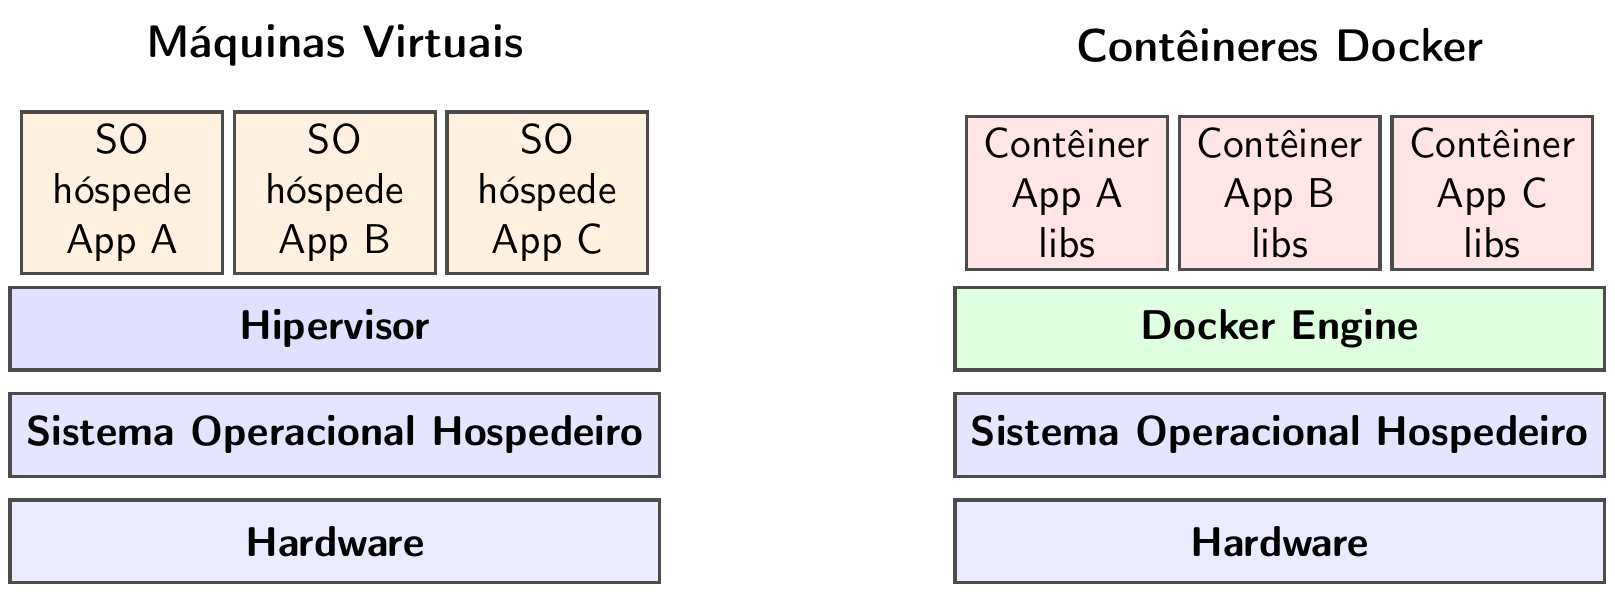
\includegraphics[width=13.62cm]{Imagens/Desenvolvimento/Cap1/vm_vs_container-nova.png}
    \vspace{0.2cm} \\
    Fonte: Elaborado pelo autor com base em \textcite{SALVADOR2019_VIRTUALIZACAO}.
\end{figure}

\par O modelo apoia-se em três artefatos \cite{DOCKER_DOCS}: o \emph{Dockerfile}, arquivo de texto que descreve como construir a imagem (base, dependências, código, inicialização); a imagem, resultado somente leitura organizado em camadas, versionável e armazenável em registros como o Docker Hub ou o Amazon ECR; e o contêiner, instância em execução de uma imagem, com seu próprio espaço de processos, rede e armazenamento volátil. A composição de múltiplos contêineres costuma ser descrita em \texttt{docker-compose.yml}, e, em produção, orquestradores como o Kubernetes ou serviços gerenciados como o Amazon ECS provisionam, monitoram, reiniciam e escalam as instâncias.

\par As vantagens são diretas para sistemas baseados em microsserviços: reprodutibilidade do ambiente (o mesmo Dockerfile gera a mesma imagem em desenvolvimento e em produção), isolamento de dependências (serviços com versões diferentes de uma biblioteca convivem sem conflito) e portabilidade (a imagem roda em qualquer ambiente com Docker Engine). Por essas razões, os contêineres tornaram-se a base de implantação das arquiteturas orientadas a microsserviços para a Indústria 4.0 \cite{BIGHETI2020}.

\subsection{Computação em Nuvem}

\par O termo \emph{Cloud Computing}, ou Computação em Nuvem, surgiu em 2006 e consolidou-se como um paradigma em que dados e aplicações são movidos para grandes centros de armazenamento e a infraestrutura é distribuída como serviços acessíveis pela internet \cite{HENRIQUES2010_CLOUD_COMPUTING_TCC}. A ``nuvem'' esconde os recursos físicos sob uma interface padronizada, em parentesco com a \emph{Utility Computing}: a capacidade computacional torna-se uma utilidade tarifada pelo consumo \cite{PEDROSA2011_COMPUTACAO_NUVEM}. Para ser considerada nuvem, uma plataforma deve reunir cinco características: \emph{self-service} sob demanda, amplo acesso à rede, \emph{pooling} de recursos multi-inquilino, elasticidade rápida e serviço medido \cite{HENRIQUES2010_CLOUD_COMPUTING_TCC,PEDROSA2011_COMPUTACAO_NUVEM}.

\par A arquitetura organiza-se em três camadas de serviço (Figura~\ref{fig:cloud_modelos_servico}): Infraestrutura como Serviço (IaaS), com recursos virtualizados de hardware; Plataforma como Serviço (PaaS), com ambientes prontos de desenvolvimento; e Software como Serviço (SaaS), com aplicações completas entregues por portais web \cite{PEDROSA2011_COMPUTACAO_NUVEM}. Quanto à implantação, há as nuvens pública, privada, comunitária e híbrida, esta última capaz de absorver picos de demanda com recursos públicos \cite{HENRIQUES2010_CLOUD_COMPUTING_TCC}.

\par Entre as vantagens estão a mobilidade, o pagamento por uso, a escalabilidade e a confiabilidade dos grandes provedores; entre os desafios, a segurança, a interoperabilidade entre provedores e a disponibilidade \cite{HENRIQUES2010_CLOUD_COMPUTING_TCC,PEDROSA2011_COMPUTACAO_NUVEM}. No contexto da Indústria 4.0, a nuvem é a infraestrutura que viabiliza a integração de produtos, máquinas, sensores e serviços, reposicionando o SCADA, antes confinado a salas de controle locais, como nó de uma rede distribuída de serviços \cite{BIGHETI2020,PISCHING2017}. Entre os provedores comerciais, a Amazon Web Services (AWS) é atualmente o maior, oferecendo serviços em todas as camadas do modelo sob precificação \emph{pay-per-use}.

\subsection{Next.js}

\par O Next.js é um \emph{framework} para a construção de aplicações web, criado sobre o React, uma biblioteca JavaScript desenvolvida pela Meta para montar interfaces a partir de componentes, isto é, pequenos blocos reutilizáveis de tela, como botões, formulários e gráficos, que se combinam para formar páginas inteiras. O React, sozinho, monta a interface diretamente no navegador do usuário: envia um arquivo quase vazio acompanhado de um programa em JavaScript que desenha a tela depois que a página carrega. Esse modelo, chamado de renderização no cliente (\emph{client-side rendering}, CSR), funciona bem, mas tem desvantagens, a primeira carga pode ser lenta e os mecanismos de busca têm dificuldade para ler o conteúdo \cite{NEXTJS_DOCS}.

\par O Next.js surge justamente para contornar essas limitações, oferecendo outras formas de gerar as páginas. Na renderização no servidor (\emph{server-side rendering}, SSR), a página já é montada pronta no servidor e enviada ao navegador, o que acelera a exibição e facilita a leitura pelos buscadores. Na geração estática (\emph{static site generation}, SSG), a página é montada uma única vez, no momento em que o sistema é publicado, e a mesma versão pronta é entregue a todos os usuários, garantindo o melhor desempenho para conteúdos que mudam pouco. Uma vantagem importante é que o Next.js permite escolher a estratégia mais adequada para cada tela, em vez de impor uma só a toda a aplicação \cite{NEXTJS_DOCS}.

\par Além das opções de renderização, o Next.js simplifica tarefas comuns do desenvolvimento. O roteamento, isto é, a associação entre os endereços (URLs) e as páginas, baseia-se na própria organização dos arquivos do projeto: cada arquivo criado em uma pasta específica vira automaticamente um endereço da aplicação, sem necessidade de configuração manual. O \emph{framework} ainda traz, de fábrica, recursos que melhoram o desempenho, como carregar apenas o código necessário a cada página, preparar de antemão as páginas que o usuário provavelmente acessará, otimizar imagens automaticamente e oferecer suporte nativo ao TypeScript, uma versão do JavaScript com verificação de tipos que ajuda a evitar erros durante o desenvolvimento \cite{NEXTJS_DOCS}.

\subsection{HTTP, API REST e JSON}

\par O protocolo HTTP (\emph{Hypertext Transfer Protocol}) é a base da comunicação na web e, por extensão, a base da comunicação entre os serviços de qualquer sistema distribuído moderno. Trata-se de um protocolo cliente-servidor sem estado (\emph{stateless}), em que cada requisição contém todas as informações necessárias para ser processada, sem dependência de requisições anteriores. Uma requisição HTTP é composta por método (GET, POST, PUT, PATCH, DELETE, entre outros), caminho do recurso (URL), cabeçalhos (\emph{headers}) e, opcionalmente, corpo (\emph{body}). A resposta contém código de status (200, 201, 400, 401, 404, 500 etc.), cabeçalhos e corpo.

\par Sobre o HTTP, o padrão REST (\emph{Representational State Transfer}), proposto por Roy Fielding em sua tese de doutorado em 2000, estabelece um conjunto de restrições arquiteturais para projetar APIs web bem comportadas. Os princípios centrais incluem: identificação clara de recursos por URL (\texttt{/equipamentos/42/tags}); uso dos métodos HTTP de forma semântica (GET para consulta, POST para criação, PUT para atualização completa, PATCH para atualização parcial, DELETE para remoção); representação independente da forma interna (frequentemente JSON na comunicação cliente-servidor moderna); ausência de estado de sessão no servidor; e estrutura hierárquica de recursos que reflete o domínio do problema. APIs REST bem desenhadas são previsíveis, navegáveis e composíveis, propriedades alinhadas com o paradigma de orientação a serviços discutido por \textcite{COLOMBO2014_STATE_ART_AUTOMATION} no contexto de automação industrial.

\par O formato JSON (\emph{JavaScript Object Notation}) é a representação de dados padrão de fato para APIs REST modernas. Trata-se de uma sintaxe textual derivada do JavaScript, simples de ler e escrever para humanos e fácil de gerar e parsear para máquinas. Suporta tipos primitivos (\emph{string}, número, booleano, nulo) e estruturas compostas (objeto e \emph{array}), o que se mostrou suficiente para a grande maioria dos cenários de troca de dados. JSON substituiu, em larga medida, o XML em comunicações web devido à sua menor verbosidade e ao acoplamento natural com o JavaScript dos navegadores. Adicionalmente, esquemas JSON (\emph{JSON Schema}) permitem descrever formalmente o formato esperado de mensagens, oferecendo validação e geração de documentação automaticamente.

\par Em sistemas industriais conectados, a comunicação por API REST sobre HTTP é hoje uma alternativa cada vez mais comum ao acoplamento direto ao protocolo Modbus. Como observa \textcite{COLOMBO2014_STATE_ART_AUTOMATION}, a exposição de funcionalidades de dispositivos de campo como serviços web (\emph{Web Services}) é um dos vetores que viabilizam o achatamento da pirâmide ISA-95.

\subsection{Microsserviços}

\par O paradigma de microsserviços é um estilo arquitetural em que a aplicação é estruturada como um conjunto de serviços pequenos, autônomos e independentemente implantáveis, cada um responsável por um domínio bem delimitado e comunicando-se por protocolos leves, tipicamente APIs HTTP/REST ou mensageria assíncrona. Popularizou-se a partir de 2014, herdeiro da \emph{Service-Oriented Architecture} (SOA) discutida por \textcite{COLOMBO2014_STATE_ART_AUTOMATION} no contexto industrial; a diferença está na granularidade e na autonomia: em vez de serviços grandes orquestrados por um barramento central, adotam-se serviços pequenos, com bancos próprios e ciclos de vida independentes.

\par A motivação vem das limitações do monolito, em que todas as responsabilidades vivem em um único processo, versionado e implantado em conjunto e escalado como um todo: à medida que cresce, a base de código fica difícil de evoluir, o tempo de implantação aumenta, uma falha pode comprometer o sistema inteiro e a escalabilidade aplica-se ao todo, não à parte realmente sobrecarregada (Figura~\ref{fig:monolito_vs_microservicos}).

\begin{figure}[H]
    \centering
    \caption{Aplicação monolítica (esquerda) versus arquitetura de microsserviços (direita)}
    \label{fig:monolito_vs_microservicos}
    \vspace{0.4cm}
    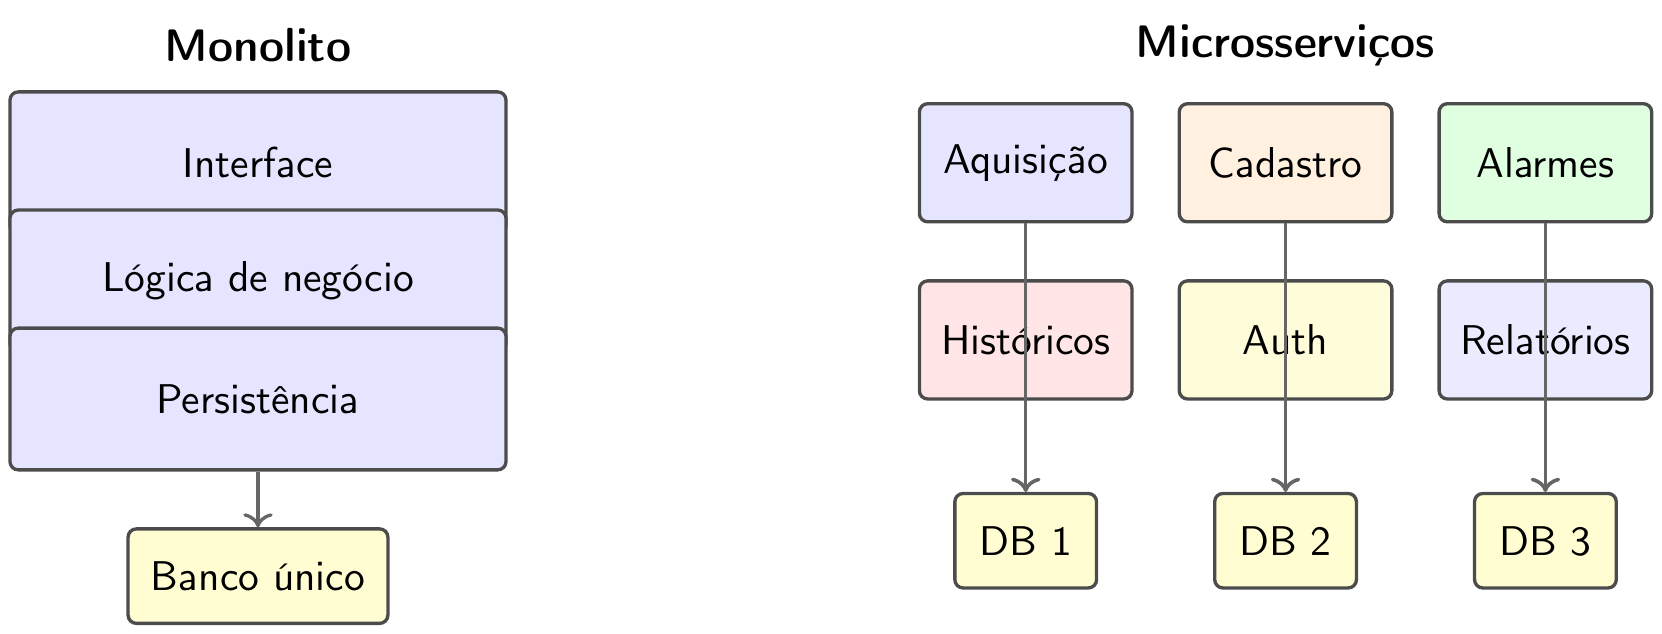
\includegraphics[width=14.02cm]{Imagens/Desenvolvimento/Cap1/monolito_vs_microservicos-nova.png}
    \vspace{0.2cm} \\
    Fonte: Elaborado pelo autor com base em \textcite{BIGHETI2020}.
\end{figure}

\par As vantagens centrais, segundo \textcite{BIGHETI2020}, são a implantação independente (cada serviço evolui sem afetar os demais), a escalabilidade granular (replica-se apenas o gargalo) e a heterogeneidade tecnológica (cada serviço usa a linguagem e o banco mais adequados). No contexto da Indústria 4.0, o autor defende que esses serviços alinham-se aos princípios de modularidade, descentralização e orientação a serviços da própria I4.0 \cite{PISCHING2017}. Há, porém, custos: a complexidade migra para o ecossistema operacional (dezenas de serviços, réplicas, observabilidade), a consistência passa a depender de mecanismos eventuais, e padrões como \emph{API Gateway}, \emph{Service Registry}, \emph{Circuit Breaker} e \emph{Distributed Tracing} tornam-se essenciais. Uma diretriz comum de decomposição é o princípio de \emph{bounded contexts} do \emph{Domain-Driven Design}, em que cada serviço corresponde a um domínio bem delimitado do problema.

\subsection{Moleculer}

\par O Moleculer é um \emph{framework} de microsserviços para Node.js, voltado a sistemas distribuídos compostos por serviços pequenos e independentemente implantáveis \cite{MOLECULER_DOCS}. Posiciona-se como alternativa pragmática a soluções mais pesadas, como o Spring Cloud no ecossistema Java, reunindo descoberta de serviços, balanceamento de carga, tolerância a falhas e diversos transportes (TCP, NATS, Redis, MQTT, Kafka) em uma única biblioteca leve.

\par No modelo do Moleculer, cada serviço define \emph{actions} (ações invocáveis remotamente, como métodos de uma API) e \emph{events} (mensagens publicadas para outros serviços), e registra-se em um \emph{broker} que faz a descoberta automática dos nós e roteia chamadas e eventos para a instância adequada, com balanceamento entre réplicas (Figura~\ref{fig:moleculer_broker}). Diante de falhas, o broker redireciona a chamada para outra instância, aplica \emph{circuit breakers} contra cascatas de falha ou retorna respostas \emph{fallback} \cite{MOLECULER_DOCS}.

\begin{figure}[H]
    \centering
    \caption{Arquitetura de microsserviços baseada em barramento de eventos (broker Moleculer)}
    \label{fig:moleculer_broker}
    \vspace{0.4cm}
    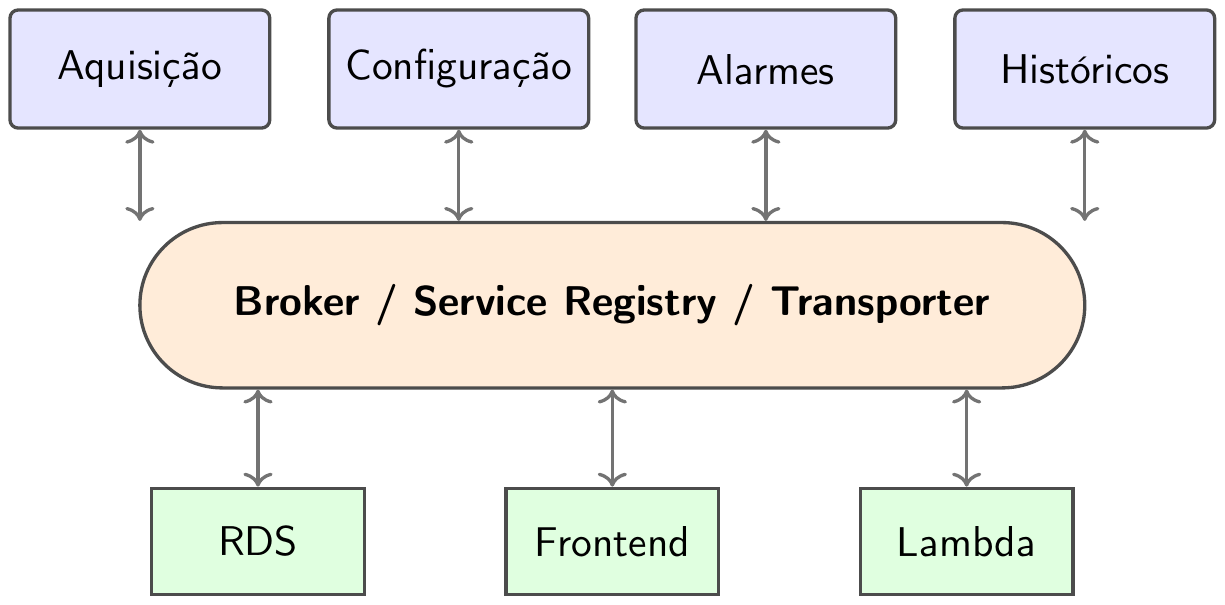
\includegraphics[width=10.33cm]{Imagens/Desenvolvimento/Cap1/moleculer_broker-nova.png}
    \vspace{0.2cm} \\
    Fonte: Elaborado pelo autor com base em \textcite{BIGHETI2020}.
\end{figure}

\par O \emph{framework} suporta múltiplos transportes: em desenvolvimento, TCP direto; em produção, barramentos resilientes como NATS, Redis Pub/Sub ou MQTT, com persistência opcional e entrega garantida. Transportes como o NATS oferecem ainda \emph{streams} persistentes, úteis para reprocessar eventos quando um serviço se recupera de falha, recurso alinhado às arquiteturas de microsserviços para a Indústria 4.0 \cite{BIGHETI2020}.

\subsection{Protocolo Modbus TCP e Modbus RTU}

\par O Modbus é um dos protocolos de comunicação mais difundidos na automação industrial. Segue o modelo de requisição e resposta entre um cliente, que faz os pedidos, e um ou mais servidores, que são os dispositivos de campo, tradicionalmente chamados de \emph{master} e \emph{slaves}. Em um sistema de supervisão, o cliente envia pedidos para ler ou escrever valores no dispositivo, e este responde com os dados solicitados ou com um código de erro quando a operação não é permitida \cite{MODBUS_TCP_IMPLEMENTATION_GUIDE}.

\par Os dados de um dispositivo Modbus ficam organizados em quatro áreas de memória: \emph{coils} e \emph{input coils}, para estados do tipo booleano, e \emph{holding registers} e \emph{input registers}, para valores numéricos de 16 bits. Cada operação é identificada por um código de função, havendo funções específicas para ler ou escrever em cada uma dessas áreas \cite{MODBUS_TCP_IMPLEMENTATION_GUIDE}.

\par Para que um valor de processo seja lido corretamente, é preciso configurar, para cada ponto, alguns parâmetros definidos pelo próprio protocolo, que indicam onde o dado se encontra no dispositivo: o endereço do dispositivo, que identifica o equipamento, o código de função, que define a área de memória e a operação, o endereço inicial e a quantidade de registradores a serem lidos. Esses parâmetros formam a base da configuração de uma \emph{tag} Modbus e permitem que um mesmo software de aquisição se comunique com medidores e controladores de fabricantes diferentes apenas alterando a configuração, sem mudar o código.

\par Além desses parâmetros do protocolo, é preciso atenção especial à forma como o dado chega, pois é nesse ponto que surgem as maiores diferenças entre fabricantes. Cada registrador Modbus tem apenas 16 bits, mas muitos valores ocupam mais espaço: um inteiro de 32 bits ou um número de ponto flutuante usam dois registradores, e um valor de 64 bits, quatro. É necessário, portanto, configurar corretamente o tipo de dado bruto e a ordem em que esses registradores e seus bytes são combinados, a chamada ordem de bytes e de palavras, que varia de um fabricante para outro e, se interpretada de forma errada, produz um valor incorreto. Por fim, quando aplicável, configuram-se os fatores de escala que convertem o valor bruto em uma grandeza de engenharia.

\par O Modbus possui duas variantes principais, que se diferenciam pelo meio de transporte. O \emph{Modbus TCP} trafega sobre redes TCP/IP, identificando o dispositivo por um endereço IP e um \emph{Unit ID}, e é comum em equipamentos com interface Ethernet. O \emph{Modbus RTU} é a forma usada em redes seriais, normalmente sobre o padrão RS-485, em que os dispositivos são identificados pelo endereço de escravo \cite{MODBUS_SERIAL_SPEC}.
